\section{Ocean Waves} \label{Ocean Waves} 
This document presents a summary of the theory of ocean waves and is mainly 
based on \cite{lewis1988principles}.

The outstanding visible characteristic of an open sea surface is its
irregularity. The waves on the surface do not repeat periodically in time or
space. Yet, over a wide area and for a period of time, the sea surface maintains
a characteristic appearance. Study on wave data have shown that even though the
sea surface is irregular, the wave elevation readings is Gaussian in nature and
is statistically a constant for a given area for a certain period of time. It is
therefore possible to define a sea condition, for a region for a (short) period
of time, using statistical parameters such as mean elevation and variance. The
mean elevation will however be zero, since wave does not change the water level
in the sea. Which means, considering Gaussian distribution for wave elevations,
the sea condition can be defined using variance alone.

For the purpose of this research we consider waves generated due to storms, that
is waves that are generated by the interaction of wind and water surface. The
two main physical process involved in the generation of storm waves are the
friction between air and water and the local variation of pressure field due to
wind. Even though there are many processes that will affect the growth and
propagation of waves, for waves of small amplitude, it is primarily governed by
the principle of superposition. So if $\zeta_1(x,y,t)$ and $\zeta_2(x,y,t)$ are
functions that represent two wave systems then $\zeta_1(x,y,t) + \zeta_2(x,y,t)$
is also a wave system.  However, it should be noted that the assumption
regarding the linear superimposability of waves fails when the wave system is
too steep and wave breaking occurs.

\subsection{Regular sea waves} \label{Regular sea waves}

A regular sea wave is a harmonic wave with crests that are infinitely long,
parallel and equally spaced and having constant wave heights. The general 
equation of a regular long crested wave travelling at a angle $\mu$ to the 
$x$-axis is:
\begin{equation}
  \zeta (x,y,t) = \zeta_a \cos[k(x \cos \mu + y \sin \mu) - \omega t + \epsilon]
  \label {eq: 2D wave equation}
\end{equation}
where: \\ 
$\zeta_a$ is the wave amplitude at the water surface\\ 
$k = \frac{2 \pi}{L_w}$ is called the wave number.\\ 
$L_w$ is the wave length\\ 
$x$ is the distance along the x-coordinate\\
$y$ is the distance along the y-coordinate\\
$\mu$ is the direction of propagation of the wave as an angle with respect to
positive direction of x-axis.\\
$\omega$ is the circular frequency of the simple harmonic wave\\
$t$ is time\\
$\epsilon$ is a phase angle. 


The wave system travels perpendicular to the line of crests with a velocity
$V_c$. It is assumed that water is incompressible and has zero viscosity. Based
on these assumptions the motion of water particle in the wave can be described
using a quantity called \textit{velocity potential} which is defined as a function
whose negative derivative in any direction yields the velocity component of the
fluid in that direction. Given
below is a simplified equation for velocity potential:
\begin{equation}
  \phi = - \zeta_a V_c \frac{\cosh k(z + h)}{\sinh k h} \sin k(x - V_c t)
  \label {eq: 2D wave velocity potential}
\end{equation}
where:\\
$h$ is the water depth (distance from sea surface to seabed)\\ 
$V_c$ is the wave velocity (or celerity)\\ 
$z$ is the vertical distance of the water particle from the surface and is 
measured positive in the upward direction\\ 
For deep water, ie. where $h \gg \frac{L_w}{2}$, 
\begin{equation}
  \frac{\cosh k(z + h)}{\sinh k h} \approx e^{k z}
  \label{eq: ratio approx for deep water}
\end{equation}
Substituting equation \ref{eq: ratio approx for deep water} in equation 
\ref{eq: 2D wave velocity potential} we get:
\begin{equation}
  \phi = - \zeta_a V_c e^{k z} \sin k(x - V_c t)
  \label{eq: 2D wave velocity potential for deep water}
\end{equation}
The wave causes variation in the distribution of pressure below the water
surface and the equation for variation of pressure head due to waves is:
\begin{equation}
  \zeta = \frac{k \zeta_a {V_c}^2}{g} \frac{\cosh k(z + h)}{\sinh k h} \cos k(x
  - V_c t)
  \label{eq: pressure head variation}
\end{equation}
For deep water the above equation can be approximated as:
\begin{equation}
  \zeta = \zeta_a e^{k z} \cos k(x - V_c t)
  \label{eq: pressure head variation for deep water}
\end{equation}
For simple harmonic motion: 
\begin{equation}
  \omega = \frac{2 \pi}{T_w} = k V_c
  \label{eq: simple harmonic motion}
\end{equation}
where $T_w$ is the time period of the simple harmonic wave.\\
Substituting equation \ref{eq: simple harmonic motion} in equations  
\ref{eq: pressure head variation} and
\ref{eq: pressure head variation for deep water}:\\
Pressure head variation due to wave for any water depth:
\begin{equation}
  \zeta = \frac{k \zeta_a {V_c}^2}{g} \frac{\cosh k(z + h)}{\sinh kh} \cos (kx
  - \omega t)
  \label{eq: pressure head variation wrt frequency}
\end{equation}
Pressure head variation due to wave for deep water:
\begin{equation}
  \zeta = \zeta_a e^{k z} \cos (k x - \omega t)
  \label{eq: pressure head variation wrt frequency deep water}
\end{equation}
The pressure at any point is given by:
\begin{equation}
  p = \rho g (-z + \zeta)
\end{equation}
\begin{equation}
  p = - \rho g z + \zeta_a \rho g e^{k z} \cos (k x - \omega t)
  \label{eq: pressure variation}
\end{equation}
The total wave energy per unit area is:
\begin{equation}
  E = \frac{1}{2} \rho g {\zeta_a}^2
  \label{eq: energy per unit area}
\end{equation}
The variance, or mean-square value of surface elevation as a function of time
is:
\begin{equation}
  S = 
  \langle\zeta (t)^2 \rangle = 
  \lim_{T \to \infty} 
  \frac{1}{T} 
  \int\limits_{-\frac{T}{2}}^{\frac{T}{2}} 
  \zeta^2(t) dt
  \label{eq: variance}
\end{equation}
For simple harmonic motion of frequency $\omega$, the above equation for 
variance can be written as:
\begin{equation}
  S(\omega) = 
  \langle\zeta (t)^2 \rangle = 
  \frac{1}{2} {\zeta_a}^2
  \label{eq: variance for simple harmonic}
\end{equation}
Based on equation \ref{eq: variance for simple harmonic}, equation 
\ref{eq: energy per unit area} can be written as:
\begin{equation}
  E = \rho g S(\omega)
\end{equation}

\subsection{Irregular sea and wave spectrum} \label{Irregular sea and wave
spectrum}

Oceanographers have found that an irregular sea wave can be resolved into a sum
of regular waves of various length and direction using Fourier Integral
techniques. Or alternatively it can be said that the visible system of waves on
the sea surface is a result of super positioning of many regular component waves
each travelling is different direction with a different amplitude, frequency,
wave length and phase. Since the component waves have different direction and
celerities, the wave patterns keeps changing with time.  It is convenient to
begin with a simple case of wave pattern observed at a single point (ie. $x = y
= 0$) and assuming that all component waves are travelling in the same direction
($\mu = 0$). Based on equation 
\ref{eq: 2D wave equation}, the simplified equation of a compound wave (ie. a 
wave that consist of many component waves) is:
\begin{equation}
  \zeta(t) = \sum _{i} (\zeta_a)_i \cos(-\omega_i t + \epsilon_i)
  \label{eq: 2D irregular wave equation}
\end{equation}

\begin{figure}
  \centering
  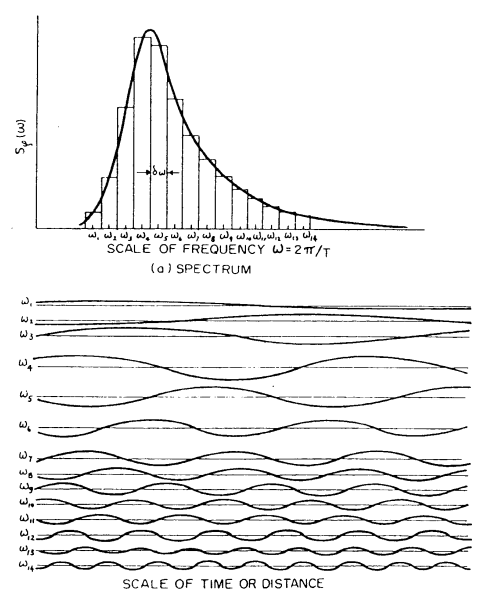
\includegraphics[scale=0.5]{variance_spectrum.png}
  \caption{Variance spectrum}
  \label{fig: variance spectrum}
\end{figure}

It is convenient to define wave components in terms of a function called 
\textit{variance spectrum, $S(\omega)$}. A typical example of a plot of variance
spectrum is shown in figure \ref{fig: variance spectrum}. For any particular 
wave frequency, $\omega_i$, the variance of the wave components for a narrow 
band of frequency, $\delta \omega$, centred on $\omega_i$ is given by:
\begin{equation}
  \langle \zeta_i (t)^2 \rangle = S(\omega_i) \delta \omega
  \label{eq: variance of a narrow band}
\end{equation}
The total variance of the system is given by:
\begin{equation}
  \langle \zeta (t)^2 \rangle = \sum _{i} \langle \zeta_i (t)^2 \rangle = 
  \int _{0}^{\infty} S(\omega) d\omega
\end{equation}
That is, the total variance of the system is obtained by finding the area under
the variance spectrum. Also, as $\delta \omega \to 0$, it means the wave system
is composed of only one frequency which means it becomes a simple harmonic wave. 
The mean value for a wave elevations for a simple harmonic wave is $0$ (wave 
does not increase the mean water level) and the variance is given by:
\begin{equation}
  \langle \zeta_i (t)^2 \rangle = \frac{1}{2} {(\zeta_a)_i }^2
\end{equation}
Applying this is equation \ref{eq: variance of a narrow band}, we get:
\begin{equation}
  \frac{1}{2} {(\zeta_a)_i}^2 = S(\omega_i) \delta \omega
\end{equation}
\begin{equation}
  (\zeta_a)_i = \sqrt{2 S(\omega_i) \delta \omega}
\end{equation}
The above equation is useful to get the amplitude of a component wave within a
frequency band. 

A fair finite-sum model of a unidirectional sea can be obtained by taking about
20 different frequency bands for a single direction. This is because any
particular rectangle in figure \ref{fig: variance spectrum} represents the
variance in that band of frequencies. A regular wave of the indicated finite
amplitude would have the same variance as the infinite number of component
within that band. Hence, the addition of these components (shown at the bottom
of the figure \ref{fig: variance spectrum}) will give a pattern that has the
same total variance and closely resemble the record from which the spectrum was
obtained.

\begin{figure}
  \centering
  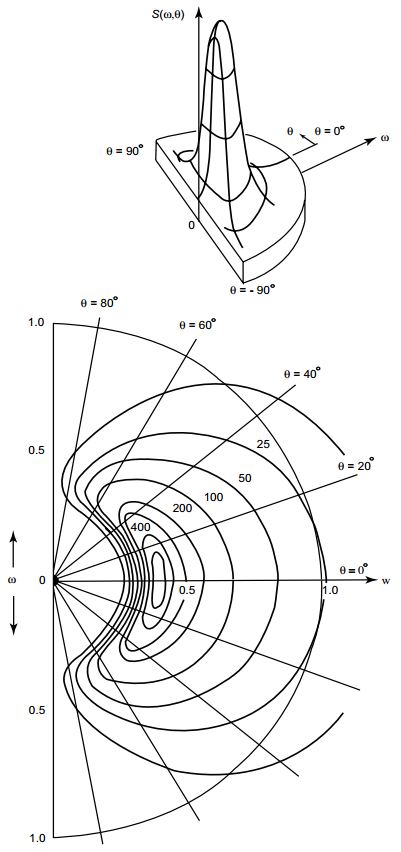
\includegraphics[scale=0.35]{directional_spectrum.png}
  \caption{Directional spectrum}
  \label{fig: directional spectrum}
\end{figure}

A point spectrum does not take into account the direction of propagation of
component waves. A \textit{directional spectrum} gives a more complete
representation of the sea. Figure \ref{fig: directional spectrum} show a typical
example of a directional spectrum. The general equation for the total wave
system of components moving in different direction, $\mu$ is:
\begin{equation}
  \zeta(x,y,t) = \sum _i \sum _j (\zeta_a)_{ij} \cos[k_i (x \cos \mu_j + 
  y \sin \mu_j) - \omega_i t + \epsilon_{ij}]
  \label{eq: equation of ocean wave system}
\end{equation}
And the total variance of the system is:
\begin{equation}
  S = \int_{0}^{\infty} \int_{0}^{2\pi} S(\omega, \mu) d\mu d\omega
  \label{eq: total variance for ocean wave system}
\end{equation}
where $S(\omega, \mu)$ is the function defining the directional spectrum such as
the one shown in figure \ref{fig: directional spectrum}. The following section
looks into various spectral families.

\subsection{Idealized spectral families} \label{Idealized spectral families}

This section describes three idealised point spectrum followed by a section
which describes how to convert point spectrum into a directional spectrum.

\subsubsection{Pierson-Moskowitz spectrum} \label{Pierson-Moskowitz spectrum}
This spectral form requires only one parameter, wind speed, as input and was
developed primarily for oceanographic use. It is intended to represent point
spectrum of a fully developed sea, that is fetch and duration are great, and
there is no contaminating swell from other areas. 
\begin{equation}
  S(\omega) = \frac{\alpha g^2}{\omega^5} 
    e^{ -\beta \big(\frac{g}{V_{\omega}} \big)^4 }
  \label {eq: pierson moskowitz spectrum}
\end{equation}
where:\\
$\omega$ is the frequency in radians/sec\\
$\alpha = 8.10 \cdot 10^{-3}$\\
$\beta = 0.74$ \\
$g =$ acceleration due to gravity in $cm/sec^2$\\
$V_{\omega} =$ wind speed in cm/sec measured 19.5m above the surface.\\

While its oceanographic importance is great, this spectral model is good only
for extreme storm condition and is inappropriate for general use because it is
based on the assumption of full developed sea state reached after an extended
time period of steady wind with no contaminating swell. 

\subsubsection{Bretschneider spectrum} \label{Bretschneider spectrum}
This spectrum takes two input parameters - wave period and wave height. It has
the form:
\begin{equation}
  S(\omega) = \frac{A}{\omega^5} e^{\frac{-B}{\omega^4}}
  \label {eq: bretschneider spectrum}
\end{equation}
where the two parameters $A$ and $B$ depend on the modal frequency, $\omega_m$,
and variance, $S$. The modal frequency is
\begin{equation}
  \omega_m = \bigg[\frac{4}{5}B \bigg]^{\sfrac{1}{4}}
\end{equation}
and total variance is 
\begin{equation}
  S = A/4B
\end{equation}
The International Towing Tank Conference (ITTC, 1978) recommends the use of a
form of Bretschneider spectrum when more specifically appropriate spectral forms
are not known. 
\begin{equation}
  A = 173 \frac{{H_{\sfrac{1}{3}}}^2 }{{T_1}^4}
\end{equation}
\begin{equation}
  B = \frac{691}{{T_1}^4} 
\end{equation}

$H_{\sfrac{1}{3}}$ is the significant wave height and $T_1$ is the time period;
both are inputs.

\subsubsection{JONSWAP spectrum} \label{JONSWAP spectrum}
This spectral function takes two parameters as input - fetch and wind speed. The 
preceding two spectrum models represent open-ocean wave conditions. However, 
this might not always be the case where geographic boundaries limit the fetch in
generating areas. North Sea is such an area and extensive oceanographic
measurements were taken under the Joint North Sea Wave Project (JONSWAP). The
spectral function derived from the recorded data is of the form: 
\begin{equation}
  S(\omega) = \frac{\alpha g}{\omega^{5}} 
  e^{
    {
    \big[ 
      -\frac{5}{4} \frac{\omega}{\omega_m} 
    \big]
    }^{-4}
  }
  \gamma^{
    e^{
        -\frac{(\omega -\omega_m)^2}{2 \sigma^2 {\omega_m}^2}
      }
    }
  \label {eq: JONSWAP spectrum}
\end{equation}
where:\\
$\gamma$ is 3.3\\
$\sigma$ is 0.07 for $\omega < \omega_m$ and is 0.09 for $\omega > \omega_m$\\
$\alpha$ is $0.076 {\tilde{x}}^{-0.22}$\\
$\omega_m $ is $ \sfrac{2 \pi \tilde{f_m} g}{V_{W10}}$ (modal frequency)\\
$\tilde{x}$ is $g \sfrac{x}{{V_{W10}}^2}$\\
$\tilde{f_m}$ is $3.5 {\tilde{x}}^{-0.33}$ \\
$x$ is fetch \\
$V_{W10}$ is wind speed at 10m (32ft) above sea level\\

Note: JONSWAP is simply a form of Bretschneider spectrum, multiplied by a
frequency dependent factor (the $\gamma$ term).

\cite{stansberg2002specialist} provides a more through listing of different wave
spectrum.

\subsubsection{Converting point spectrum to directional spectrum}
\label{Converting point spectrum to directional spectrum}
According to \cite{stansberg2002specialist} even though there are several
unidirectional spectral models, there are only a few multidirectional spectral
models. But, for the multidirectional wave models that are available, the 
data documentation has been lacking or is uncertain. In addition
\cite{stansberg2002specialist} also mentions that for modelling purpose, the
directional characteristics of waves are assumed to be uncoupled from their
spectral properties, and the spectrum of waves travelling within a given range
of headings is taken to be some proportion of that measured at a point. On this
basis, the directional spectrum is of the form:
\begin{equation}
  S(\omega, \mu) = S(\omega) G(\mu)
\end{equation}
$G(\mu)$ is called the \textit{spreading function} and is of the form:
\begin{equation}
  G(\mu) = F(s) \cos^{2s} \frac{1}{2} (\mu - \mu_1)
\end{equation}
where:\\ 
$\mu_1$ is the predominant wave direction  \\
$s$ is an index that determines the width of the directional spread.
\begin{equation}
  F(s) = \frac{2^{2s - 1}}{\pi} \frac{\Gamma^2 (s+1)}{\Gamma (2s + 1)}
\end{equation}
$\Gamma$ is the Gamma function. The function $F(s)$ ensures that the total
variance of the directional spectrum $S(\omega, \mu)$ is same as that of the
point spectrum $S(\omega)$ from which it is derived.\\
\textbf{Note:} Could not find appropriate value for the index $s$ in ITTC 
recommendations.


DNV-GL-H103 \cite{dnv2014recommended} (section 2.2.7) also suggests a similar
approach for converting a point spectrum to a directional spectrum. 
\begin{equation}
  S(\omega, \mu) = S(\omega) G(\mu)
\end{equation}
\begin{equation}
  G(\mu) = \frac{\Gamma(1 + \sfrac{n}{2})}
                {\sqrt{\pi} \Gamma(\sfrac{1}{2} + \sfrac{n}{2})}
           \cos^n (\mu - \mu_p)
\end{equation}
where $\mu_p$ is the prevailing wind direction.

An alternative to the above two formulation is the $15^{th}$ ITTC (1978) 
recommendation mentioned in \cite{lewis1988principles}.
\begin{equation}
  G(\mu) = k \cos^n \mu
\end{equation}
where: \\ 
$\sfrac{-\pi}{2} < \mu < \sfrac{\pi}{2}$\\ 
$n = 2$ \\
$k = \sfrac{2}{\pi}$



